\documentclass[conference]{IEEEtran}
\IEEEoverridecommandlockouts
% The preceding line is only needed to identify funding in the first footnote. If that is unneeded, please comment it out.
\usepackage{cite}
\usepackage{amsmath,amssymb,amsfonts}
\usepackage{algorithmic}
\usepackage{graphicx}
\graphicspath{ {../images/} }
\usepackage{textcomp}
\usepackage{xcolor}
\def\BibTeX{{\rm B\kern-.05em{\sc i\kern-.025em b}\kern-.08em
    T\kern-.1667em\lower.7ex\hbox{E}\kern-.125emX}}

\begin{document}

\title{Stock Price Prediction using Machine Learning Models}

\author{\IEEEauthorblockN{1\textsuperscript{st}Geoff Patton, 2\textsuperscript{nd}Rohit Bhattacharya, 3\textsuperscript{rd}Fengtian Lu, 4\textsuperscript{th}Ananda Mahalingam }
\IEEEauthorblockA{
\textit{College of Computing \& Informatics}\\
\textit{Drexel University}\\
Philadelphia, United States \\
gp495@drexel.edu, rb689@drexel.edu, fl373@drexel.edu, asm465@drexel.edu}
}

\maketitle

\begin{abstract}
Prediction of stock prices has been a major area of research for a long time.
While supporters of the efficient market hypothesis believe that it is impossible to predict stock prices accurately, there are formal propositions demonstrating that accurate modeling and designing of appropriate variables may lead to models using which stock prices and stock price movement patterns can be very accurately predicted.
This paper attempts to predict stock price of few ticker symbols to prove the theory.
We propose an approach of modeling for stock price prediction for CMCSA (Comcast) and its competitors building different machine learning and deep learning-based models.
This paper also attempts to compare the price prediction from different models for different ticker symbols.
The Data collected from Finn Hub using the Finn Hub APIs, preprocessed, and prepared for training the model.
The Dataset will be split into 80\%-20\% split with 80\% of the data used for training the model.
The following models are used for predicting the stock price among others: Linear regression, locally weighted Linear regression, Decision Tree Regression and Random Forest Regressor.
This paper lays out the results from different models, provides an accuracy score for each model and provides insight into the best fit for the stock price prediction.
\end{abstract}

\section{Background}

Comcast Corporation operates as a media and technology company worldwide.
It operates through Residential Connectivity \& Platforms, Business Services Connectivity, Media, Studios, and Theme Parks segments.
The Residential Connectivity \& Platforms segment provides residential broadband and wireless connectivity services, residential and business video services, advertising sales, and Sky channels. Some of the top competitors of Comcast include Verizon, AT\&T, Charter Communications, Dish Network, and Walt Disney Company.
Comcast stock is listed in the NASDAQ stock exchange using the symbol (CMCSA).\par
Machine learning is a branch of artificial intelligence that analyzes complex sets of historical data, discovers hidden relationships between data sets, makes forecasts, and learns along the way to become even more accurate.
Such capabilities make ML-based tools well-suited for financial analysis.
Machine learning (ML) is playing an increasingly significant role in stock trading.
Predicting market fluctuations, studying consumer behavior, and analyzing stock price dynamics are examples of how investment companies can use machine learning for stock trading.\par
In this paper, we shall use the machine learning models to predict the stock price of Comcast (CMCSA) and one of its prime competitors, Verizon (VZ).
The predicted price can then be compared with the actual stock price to arrive at an accuracy score. Regression is a key element of predictive modelling and is a perfect fit for predicting financial stock prices.
We will be using various regression models for our study here.

\section{Related Work}

Mehar Vijh, Deeksha Chandola, Vinay Anand Tikkiwal, and Arun Kumar tested Random Forest along with neural networks using 4 features (\,Open, High, Low, and Close)\, using the Root Mean Squared Error (RMSE) and the Mean Absolute Percentage Error (MAPE) metrics as indicators and found that they were effective in predicting the stock prices \cite{b3}.
Mehtabhorn Obthong, Nongnuch Tantisantiwong, Watthanasak Jeamwatthanachai and Gary Wills used various ML techniques partially focused on regression to predict stock prices including KNN, Neural Networks and Random Forest \cite{b4}.
Ramkrishna Patel, Vikas Choudhary, Deepika Saxena, and Ashutosh Kumar Singh discussed feature reduction in data pre-processing in application of different approaches including Naïve Bayes, KNN, and Linear Regression to predict stock prices \cite{b5}.

\section{Methodology}

\subsection{Data Collection using Finnhub}

Over the last few years, several new market data providers have come online. They tend to have modern websites, broad coverage, and well-documented RESTful APIs.
Their services are often priced very competitively - especially for personal use - and usually have generous free tiers.
One such newcomer is finnhub.io. Its offering includes stock, bond, crypto, and FX historical price data and real time trades and quotes.
Their fundamental data offering is noticeably broad and includes current values and point-in-time snapshots for numerous metrics.
There are also some interesting alternative data sets including measures of social media sentiment, insider transactions and insider sentiment, senate lobbying, government spending, and others.
In addition, there is a real-time newsfeed delivered over web-sockets.\par
Our dataset for this research activity has been prepared using FinnHub free tier.
The free tier is quite generous and offers more than enough for doing proof of concept work and testing ideas.
It contains quite a few Rest API endpoints and allows 60 calls per minute.
However, some of the data is limited when using the free tier.
For example, the candlestick data that provides the daily stock price only contains 1 year of historical data.
For this analysis, we are using the financial data for Comcast (CMCSA) and a few of its competitors from various segments such as internet/broadband, media, mobile, gaming, etc.
The competitors included in this paper include Verizon (VZ), AT\&T (T), and Dish Network (DISH).

\subsection{Data Preprocessing}
Data preprocessing is a step in the data mining and data analysis process that takes raw data and transforms it into a format that can be understood and analyzed by computers and machine learning.
Good, preprocessed data is even more important than the most powerful algorithms, to the point that machine learning models trained with bad data could be harmful to the analysis.

\subsubsection{Handling Missing Data}
Missing values are one of the common issues in machine learning models, and their causes are related to human errors, interruptions in the data flow, and incorrect measurements, among others.
Most of the algorithms in machine learning do not accept missing values and through errors if a dataset has missing values.
Therefore, it is necessary to solve this issue utilizing some mechanism to deal with or remove them.
Removing rows or columns with missing data can affect the performance of the model, as the size of the data decreases.

\subsubsection{Handling Outliers}
Outliers can be detected by plotting the distribution of the returns and observing if the distribution has extreme fat tails, which is a hint of some anomaly in the data.
Also, outliers can be detected by using the percentiles of the data.
Researchers can define a certain percentage threshold in the upper bottom of the distribution where values beyond these limits are considered outliers.

\subsubsection{Scaling}
After scaling a dataset, all the continuous variables become identical in terms of the range.
It is required to scale all the inputs to have values that can be compared.
Some techniques to scale values on a dataset are Normalization and Standardization.

\subsubsection{Normalization}
Normalization scales all values in the range 0 and 1.
Each value of the variable is subtracted by the min value and divided by the difference between the max value and the min value.
The procedure does not change the distribution of the feature.
Before normalization, outliers should be handled.

\begin{equation}
    Xnorm = \frac{X - X_{\min}}{X_{\max} - X_{\min}}
\end{equation}

\subsubsection{Standardization}

This method is also called the z-score and scale each of the values of a column by removing from them the mean of the column and divided by the standard deviation.
This technique decreases the effect of outliers in each feature.

\begin{equation}
    Z = \frac{x - \mu}{\sigma}
\end{equation}


\subsection{Data Analysis}

The FinnHub Free tier APIs provides one year of candlestick data for stocks.
This data set contains the daily open, high, low, close, and volume values (OHLCV) of a stock over time.

\begin{figure}
    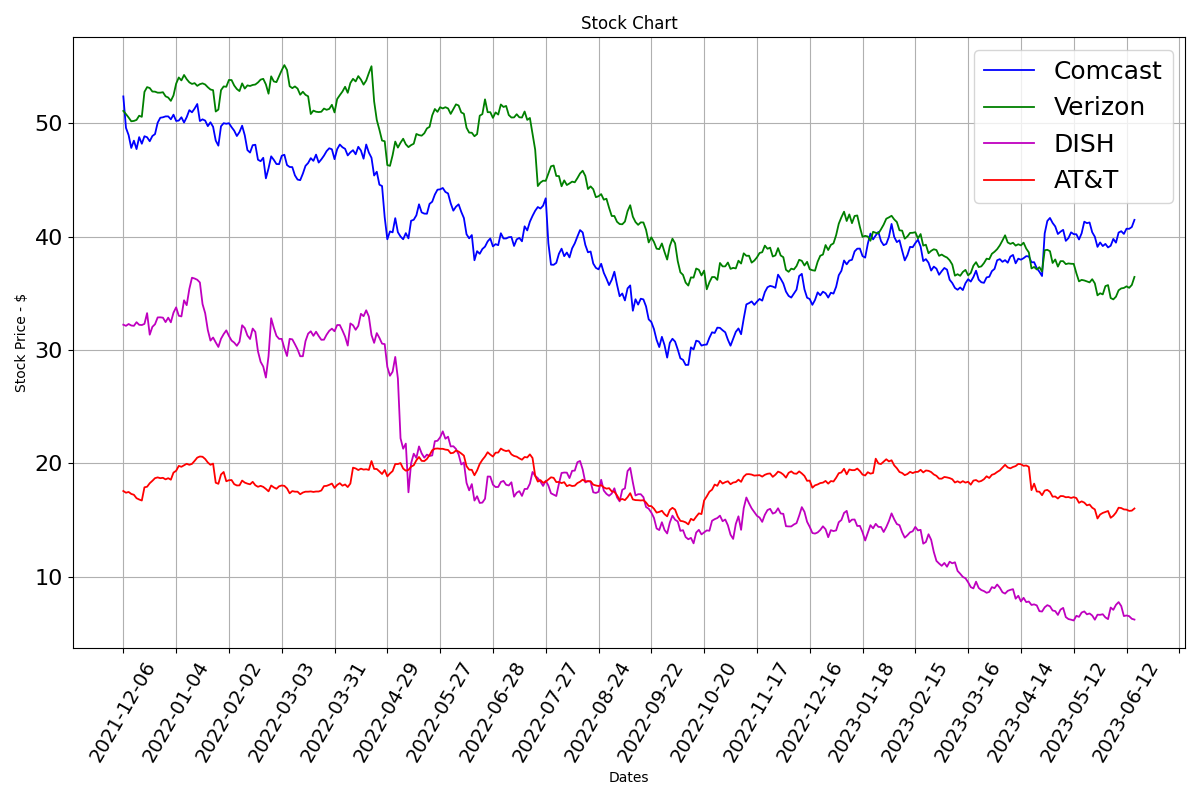
\includegraphics[width=\columnwidth]{stock_chart}
    \caption{This shows the stock price history for Comcast and its competitors over the last year and a half.}
\end{figure}

\begin{figure}
    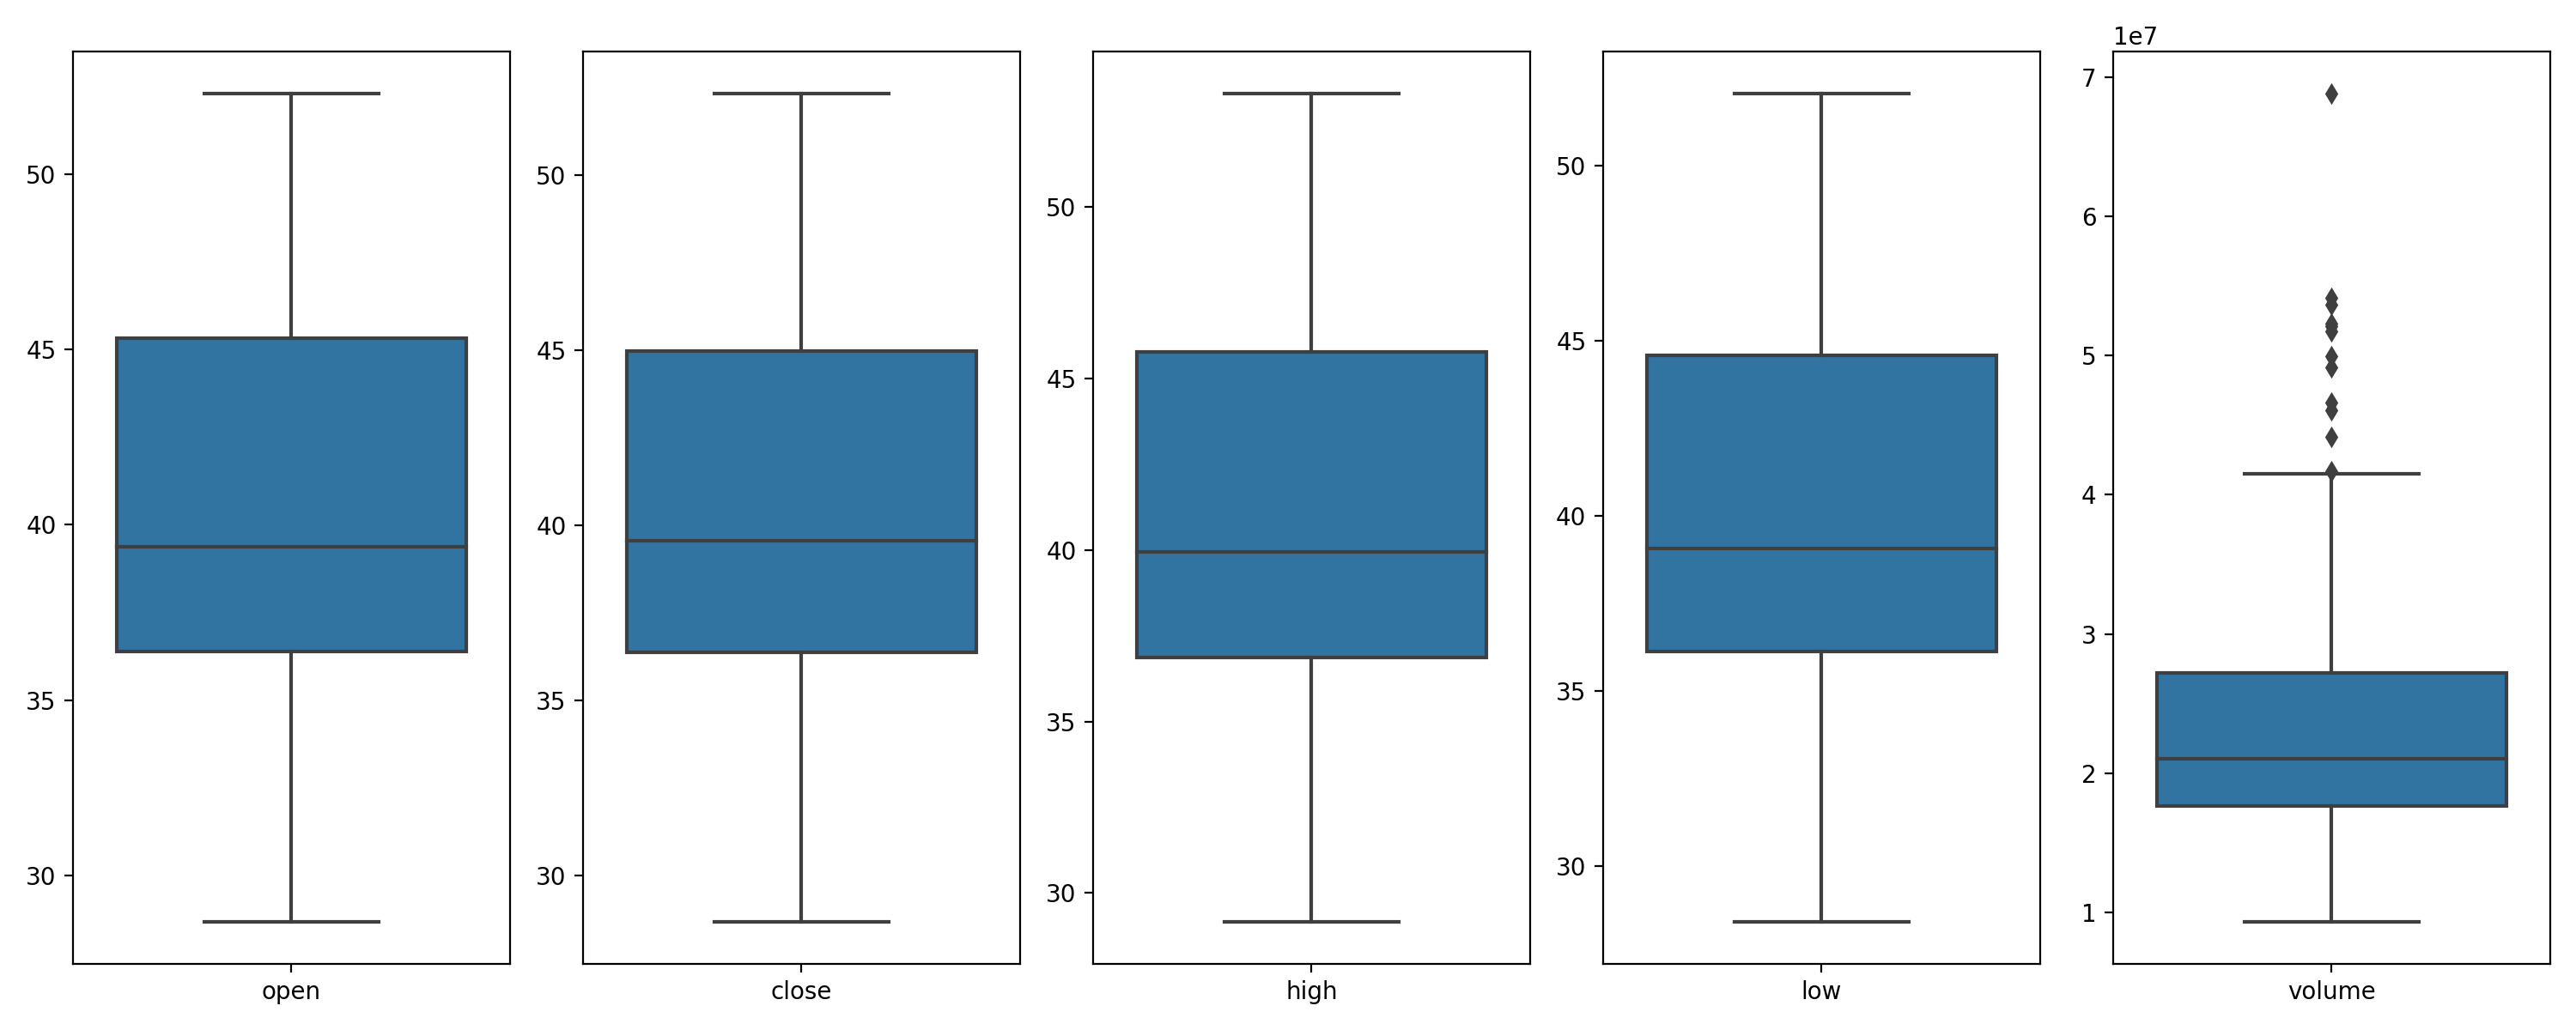
\includegraphics[width=\columnwidth]{data_distribution}
    \caption{This shows the distribution of the candlestick data for the CMCSA ticker symbol.}
\end{figure}

\subsection{Machine Learning Models} \label{sec:models}

\subsubsection{Linear Regression}
Linear regression attempts to model the relationship between two variables by fitting a linear equation to observed data.
One variable is considered an explanatory variable, and the other a dependent variable.
It must be determined if there is a relationship between the variables of interest.
A scatterplot can be a helpful tool in determining the strength of the relationship between two variables.
If there appears to be no association between the proposed explanatory and dependent variables, then fitting a linear regression model to the data will not provide a useful model.
A linear regression line has an equation of the form below:

\begin{equation} \label{eq:lr}
    Y = a + bX
\end{equation}

In equation \ref{eq:lr}, X is the explanatory variable and Y is the dependent variable.
b is the slope and a is the intercept (value of y when x = 0).

\subsubsection{Locally Weighted Linear Regression}
Locally Weighted Linear Regression (LWLR) is a non-parametric regression technique that fits a linear regression model to a dataset by giving more weight to nearby data points.
LWLR fits a separate linear regression model for each query point based on the weights assigned to the training data points.
The weights assigned to each training data point are inversely proportional to their distance from the query point.
Training data points that are closer to the query point will have a higher weight and contribute more to the linear regression model.
LWLR is useful when a global linear model does not capture the relationship between the input and output variables.
The goal is to capture local patterns in the data.
(Figure \ref{fig:lwlr})

\subsubsection{K-Folds Cross Validation}
Cross-validation is a resampling procedure used to evaluate machine learning models on a limited data sample.
The procedure has a single parameter called k that refers to the number of groups that a given data sample is to be split into. As such, the procedure is often called k-fold cross-validation.
When a specific value for k is chosen, it may be used in place of k in reference to the model, such as k=20 becoming 20-fold cross-validation.
Cross-validation is primarily used in applied machine learning to estimate the skill of a machine learning model on unseen data.
That is, to use a limited sample to estimate how the model is expected to perform in general when used to make predictions on data not used during the training of the model.
(Figure \ref{fig:kflr})

\subsubsection{Decision Tree Regressor}
Decision trees build regression or classification models in the form of a tree structure.
It breaks down a dataset into smaller subsets while an associated decision tree is incrementally developed.
The result is a tree with decision and leaf nodes.
A decision node has two or more branches, each representing values for the attribute tested.
The leaf node represents a decision on the numerical target.
The topmost decision node in a tree which corresponds to the best predictor is called root node.
Decision trees can handle both categorical and numerical data.
(Figure \ref{fig:dt})

\subsubsection{Random Forest Regressor}
Random Forest is a ensemble technique capable of performing both regression and classification tasks with the use of multiple decision trees and a technique called Bootstrap and Aggregation, commonly known as bagging.
The basic idea behind this is to combine multiple decision trees in determining the final output rather than relying on individual decision trees.
Random Forest has multiple decision trees as base learning models.
We randomly perform row sampling and feature sampling from the dataset forming sample datasets for every model.
This part is called Bootstrap.
(Figure \ref{fig:rf})

\subsubsection{Gradient Boosting}
Gradient boosting is a machine learning technique used in regression and classification tasks, among others.
It gives a prediction model in the form of an ensemble of weak prediction models, which are typically decision trees.
When a decision tree is the weak learner, the resulting algorithm is called gradient-boosted trees; it usually outperforms random forest.
A gradient-boosted trees model is built in a stage-wise fashion as in other boosting methods, but it generalizes the other methods by allowing optimization of an arbitrary differentiable loss function.
(Figure \ref{fig:gb})

\subsubsection{Bayesian Ridge}
Bayesian regression is a type of linear regression that uses Bayesian statistics to estimate the unknown parameters of a model.
It uses Bayes theorem to estimate the likelihood of a set of parameters given observed data.
The goal of Bayesian regression is to find the best estimate of the parameters of a linear model that describes the relationship between the independent and the dependent variables.
The main difference between traditional linear regression and Bayesian regression is the underlying assumption regarding the data-generating process.
Traditional linear regression assumes that data follows a Gaussian or normal distribution, while Bayesian regression has stronger assumptions about the nature of the data and puts a prior probability distribution on the parameters.
(Figure \ref{fig:bay_ridge})

\subsection{Experiment and Results}

The predicted and actual stock prices comparison for the last 8 months can be viewed in Figure \ref{fig:lr}-\ref{fig:bay_ridge} for the models described in \ref{sec:models}.
The precision for each model is displayed in the Metrics Table in Figure \ref{fig:metrics}.
The metrics include the R-squared score, Mean Squared Error (\ref{eq:mse}), Mean Absolute Error (\ref{eq:mae}), and the Mean Absolute Percentage Error.

\begin{equation}
    \sum_{i=1}^{D}(x_i-y_i)^2
    \label{eq:mse}
\end{equation}

\begin{equation}
    \sum_{i=1}^{D}|x_i-y_i|
    \label{eq:mae}
\end{equation}

The regression models perform well for the most part apart from minor variations at certain points.

\begin{figure}[b]
    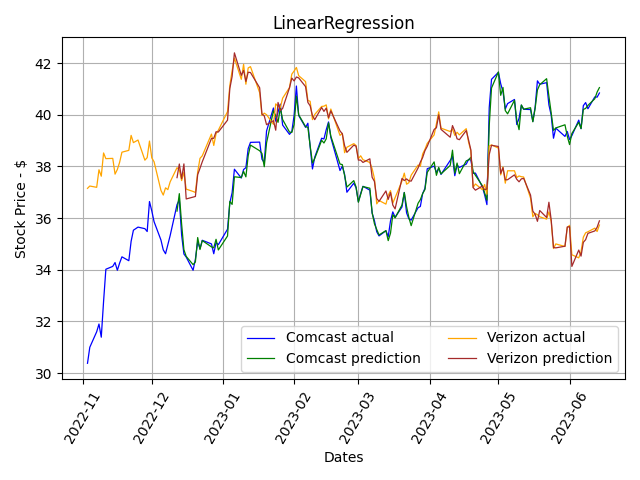
\includegraphics[width=\columnwidth]{LinearRegression}
    \caption{Basic Linear Regression}
    \label{fig:lr}
\end{figure}

\begin{figure}
    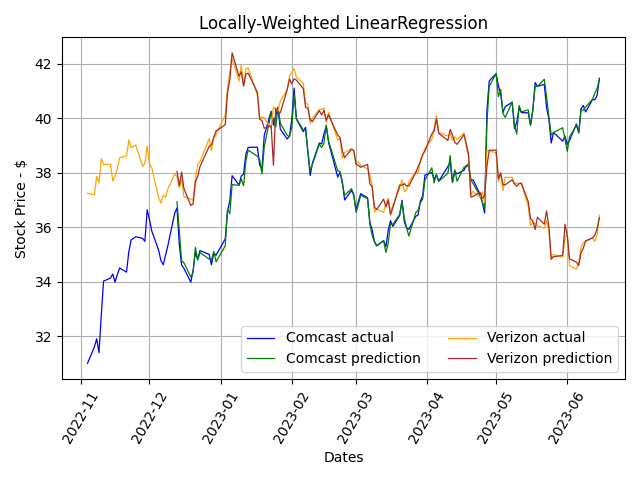
\includegraphics[width=\columnwidth]{Locally-Weighted LinearRegression}
    \caption{Locally-Weighted Linear Regression}
    \label{fig:lwlr}
\end{figure}

\begin{figure}
    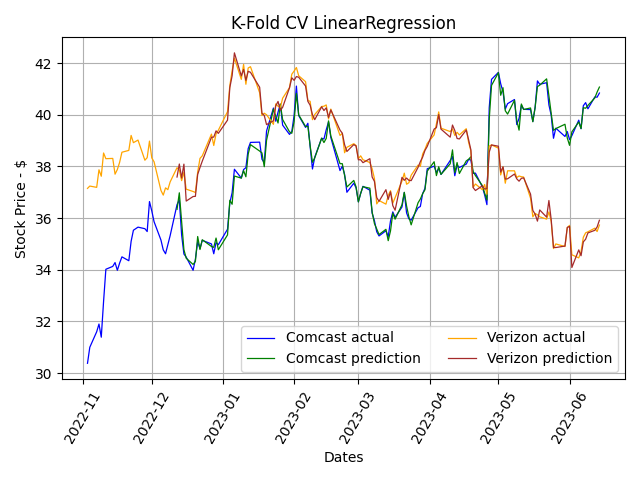
\includegraphics[width=\columnwidth]{K-Fold CV LinearRegression}
    \caption{Linear Regression with K-Fold Cross Validation}
    \label{fig:kflr}
\end{figure}

\begin{figure}
    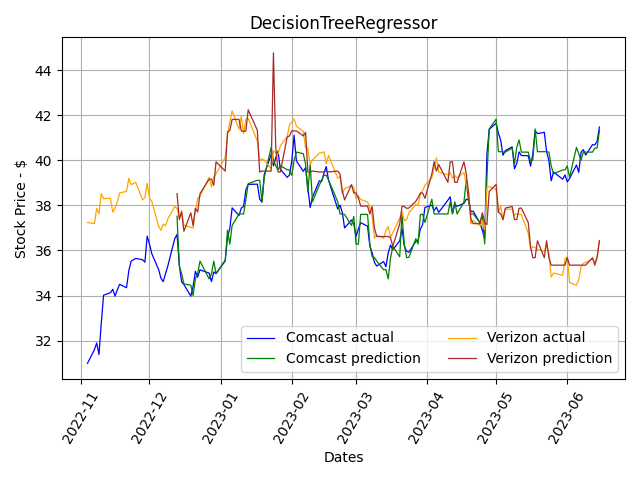
\includegraphics[width=\columnwidth]{DecisionTreeRegressor}
    \caption{Decision Tree Regressor}
    \label{fig:dt}
\end{figure}

\begin{figure}
    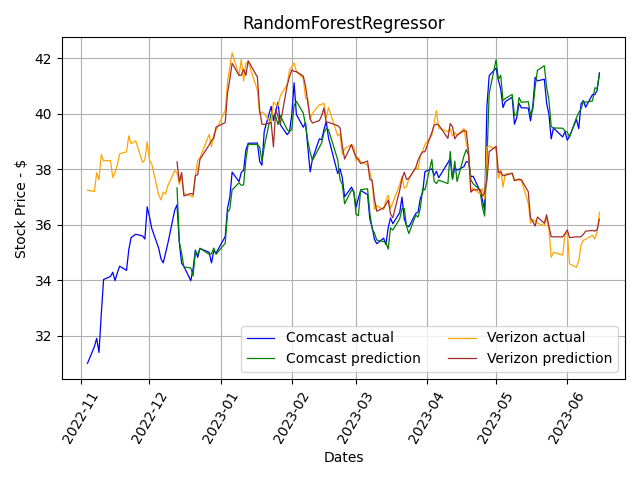
\includegraphics[width=\columnwidth]{RandomForestRegressor}
    \caption{Random Forest Regressor}
    \label{fig:rf}
\end{figure}

\begin{figure}
    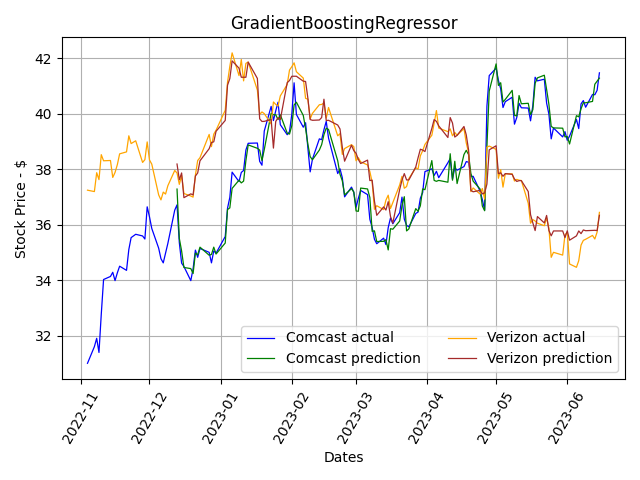
\includegraphics[width=\columnwidth]{GradientBoostingRegressor}
    \caption{Gradient Boosting Regressor}
    \label{fig:gb}
\end{figure}

\begin{figure}
    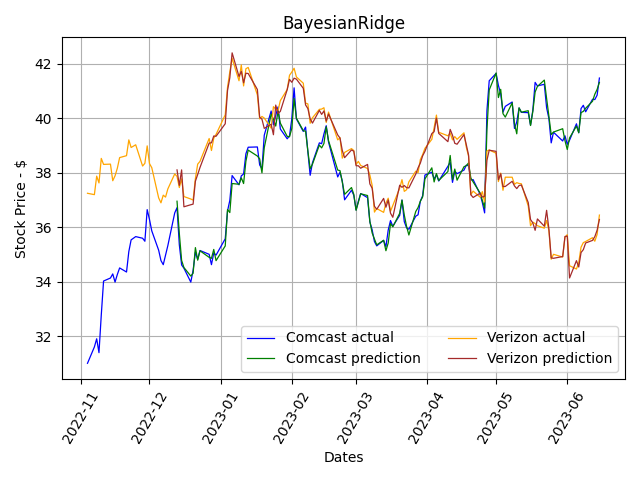
\includegraphics[width=\columnwidth]{BayesianRidge}
    \caption{Bayesian Ridge Regressor}
    \label{fig:bay_ridge}
\end{figure}

\begin{figure}
    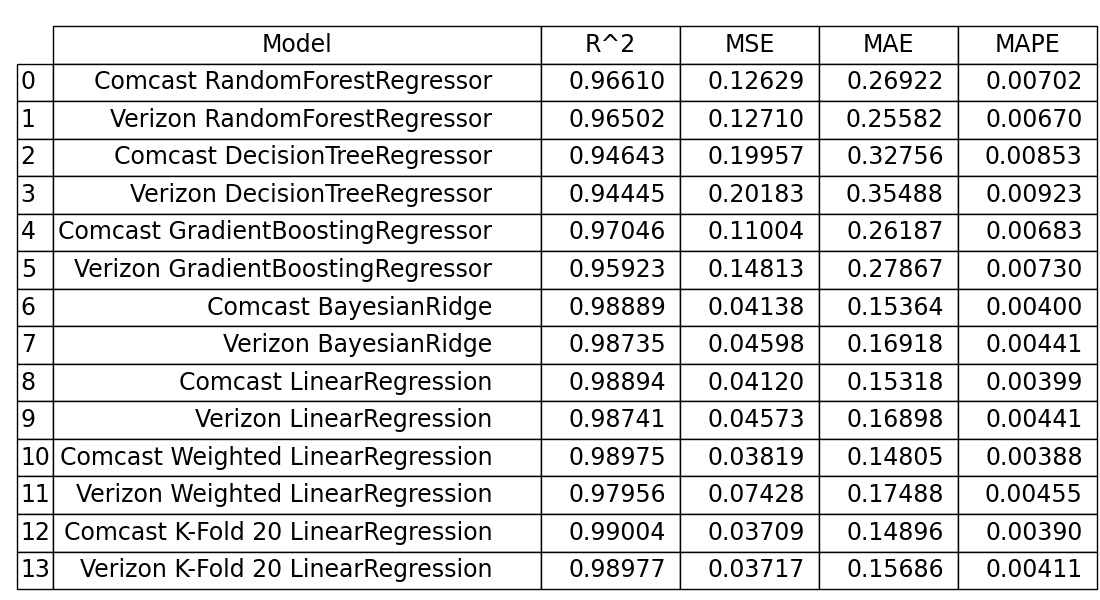
\includegraphics[width=\columnwidth]{metrics}
    \caption{Metrics for each model. Including the R-squared score, Mean Squared Error (MSE),
    Mean Absolute Error (MAE), Mean Absolute Percentage Error (MAPE)}
    \label{fig:metrics}
\end{figure}


\section{Conclusion}

In this paper, we have tried to apply the machine learning models to predict the stock price of Comcast and Verizon.
The Stock prediction is a regression problem and hence we have chosen various regression models to predict the stock price.
For our experiment, the Data set was obtained using the Finn Hub Free tier APIs and we could only get the data for the last one year.
With subscription, Finn Hub provides the entire data set including historical data for the last 10 years. The data set was split into 80\% training and 20\% testing set.
The training set was used to train the model and then use the testing set to predict the stock price. The predicted results are then compared with the actual stock price to calculate the accuracy. Based on the results, all the regression models provide an accuracy of above 90\% but the linear regression models provide an accuracy of above 98\%.
Hence, we conclude that linear regression is the most appropriate model for predicting stock prices.\par
We could add additional features to the training set such as other financial data, stock market sentiment data etc., and improve the accuracy score. Despite the constraints with the limited data set, the initial results show that the linear regression can be used to accurately predict the stock prices.

\section{Future Work}
The next steps of development would be to predict the future direction of a stock.
We can accomplish this by applying some supervised learning methods shown here and incorporating additional financial market data.
Another approach would be to train a neural network that will predict the close price for the next day using our existing dataset. \cite{b1}
Below are examples of the financial market data that could be included in our dataset to train the model.


\begin{figure}
    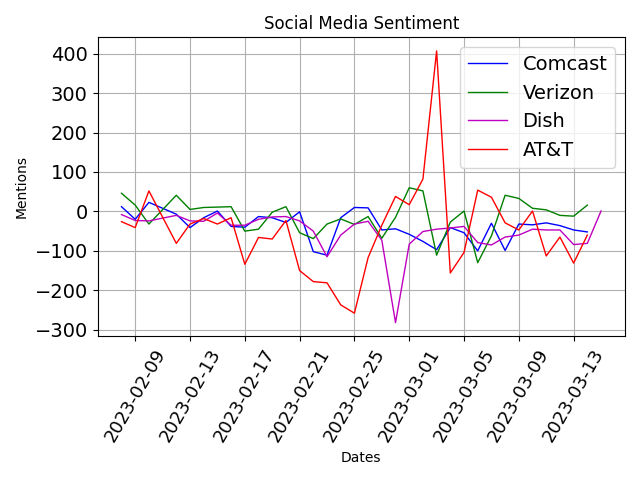
\includegraphics[width=\columnwidth]{social_media_sentiment}
    \caption{Social media sentiment over time for Comcast and its competitors.}
\end{figure}

\begin{figure}
    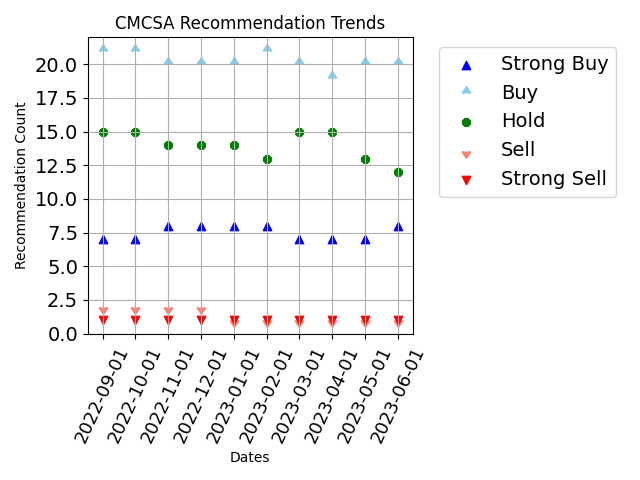
\includegraphics[width=\columnwidth]{trends}
    \caption{Monthly stock analyst recommendation for Comcast.}
\end{figure}

\begin{figure}
    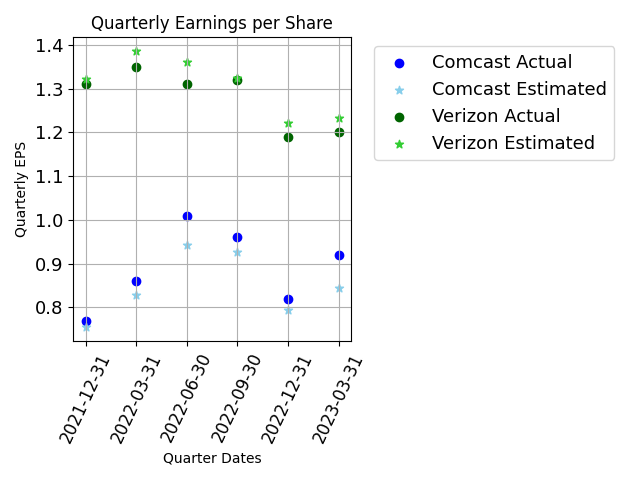
\includegraphics[width=\columnwidth]{earnings}
    \caption{Quarterly Estimated vs Actual Earnings per Share for Comcast and Verizon.}
\end{figure}

\begin{figure}
    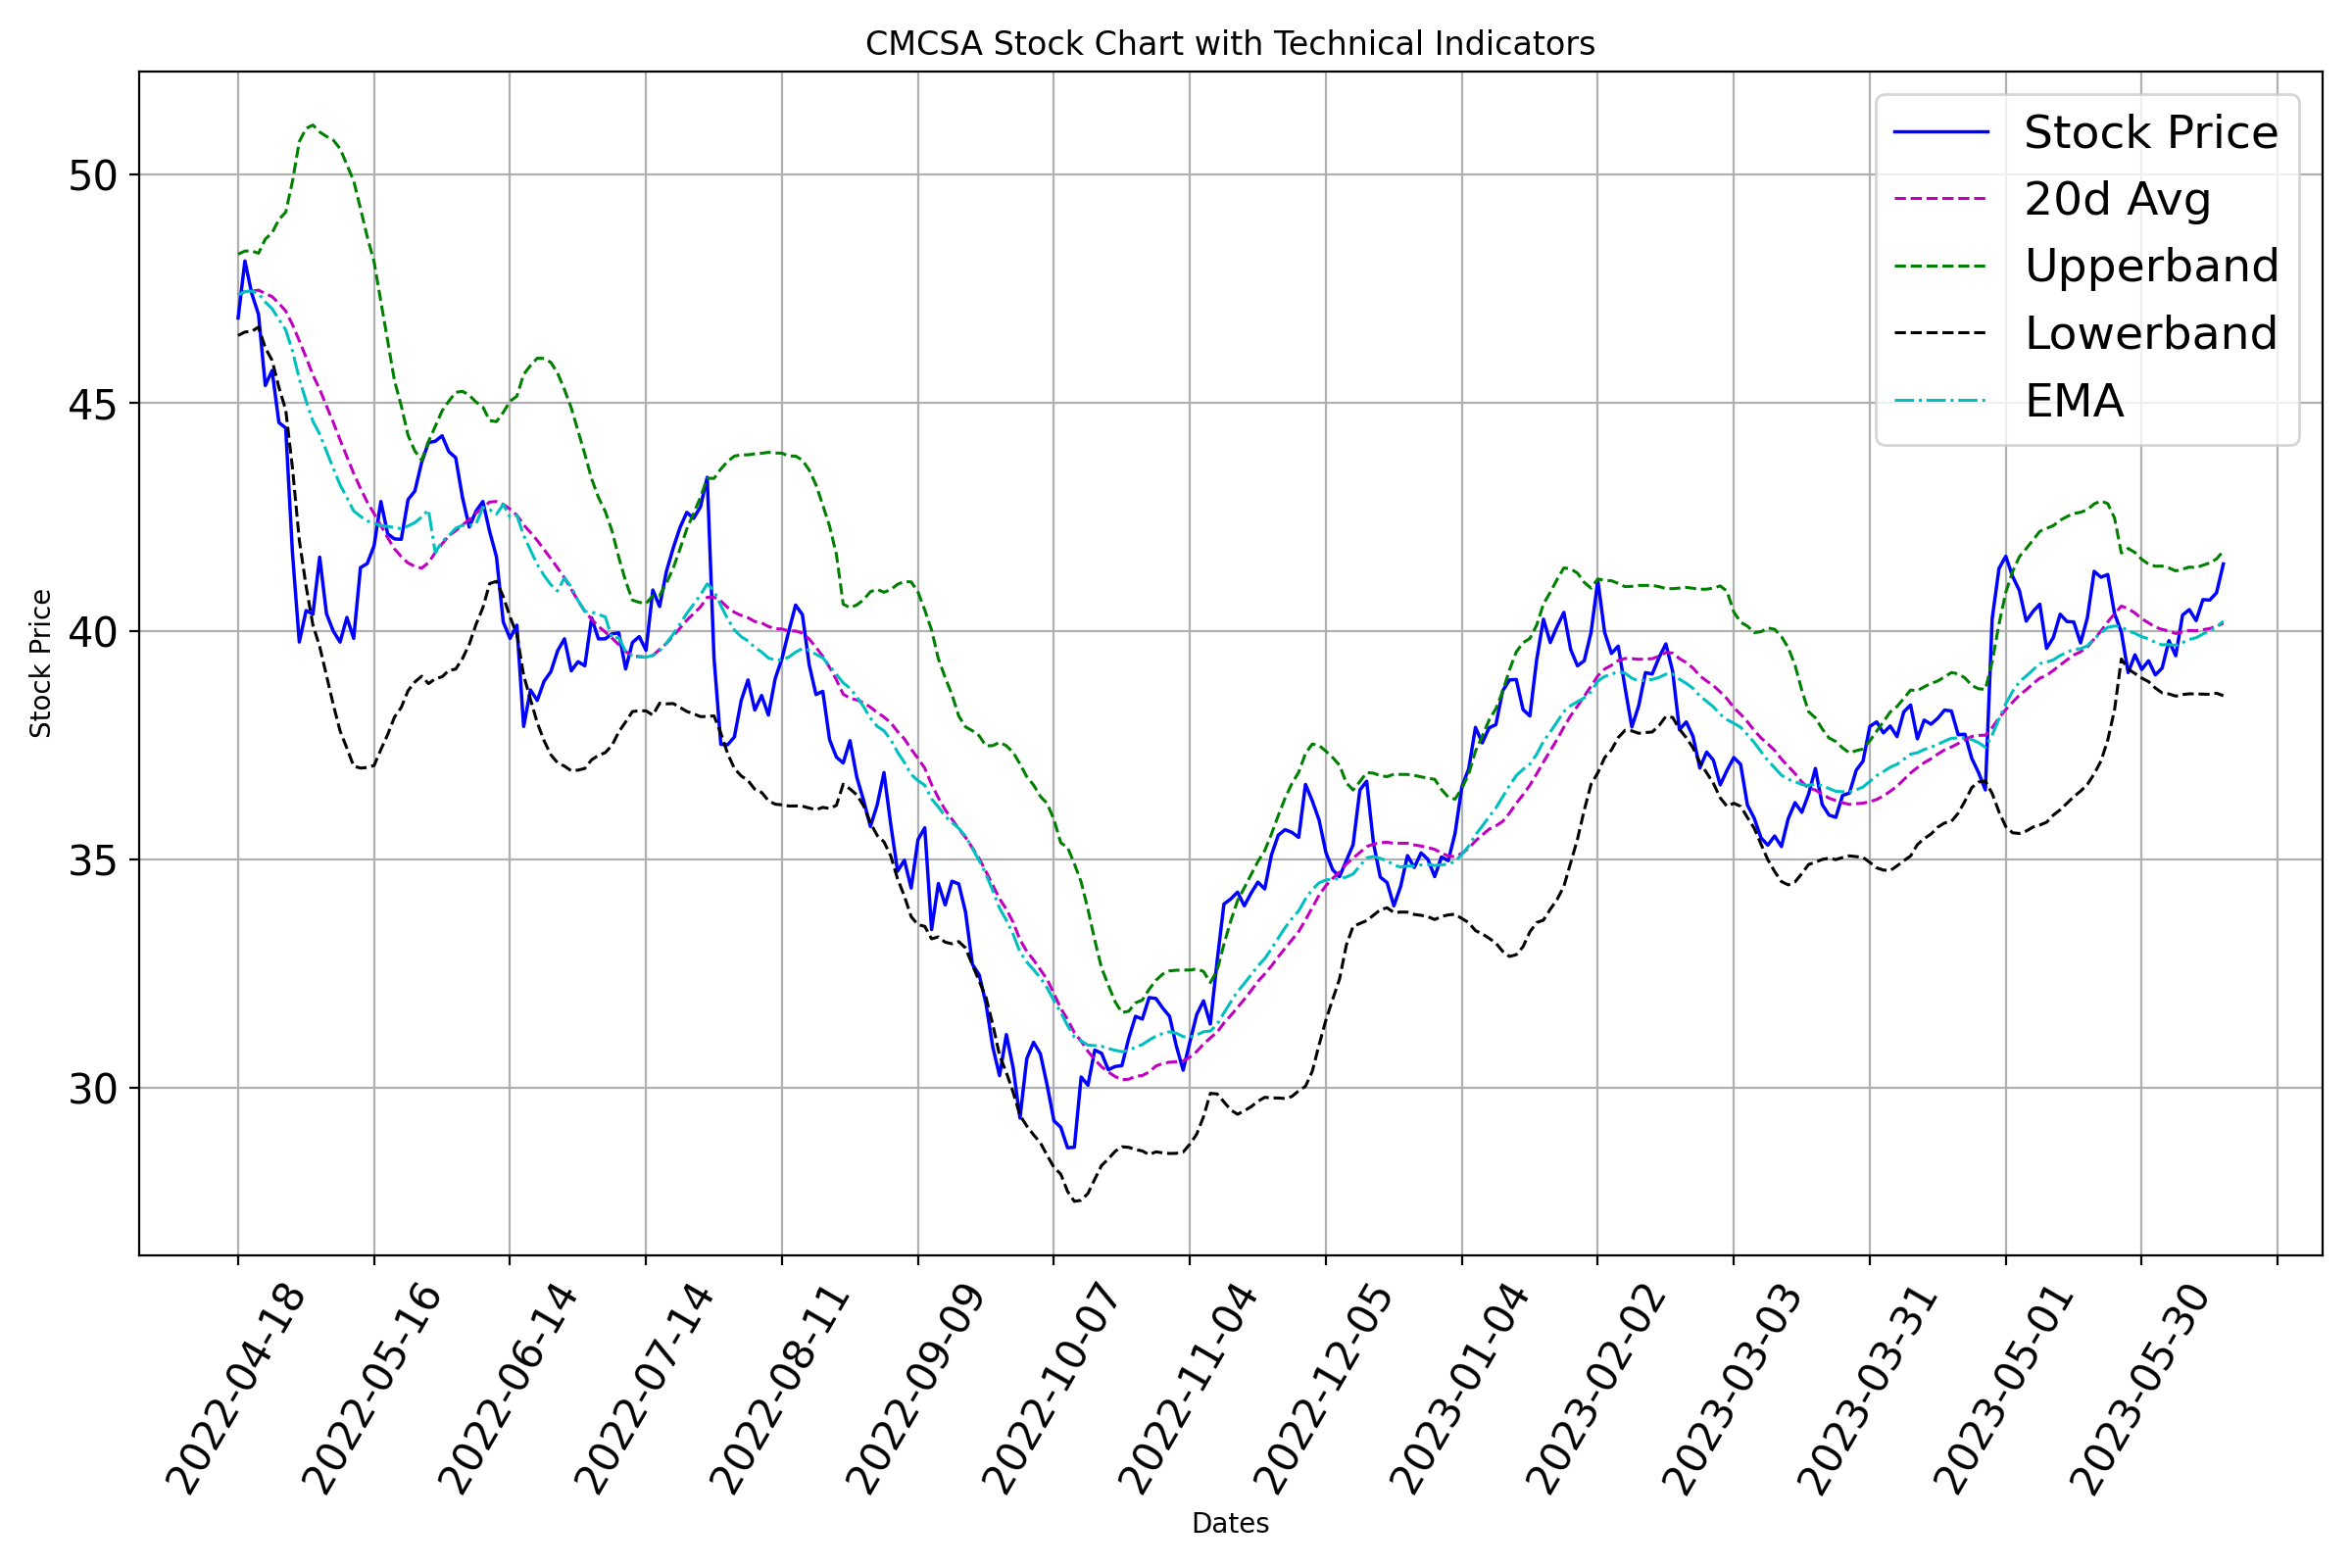
\includegraphics[width=\columnwidth]{tech_indicators}
    \caption{Stock Chart with Technical Indicators}
\end{figure}

\section*{Bibliography}

\begin{thebibliography}{00}
\bibitem{b1} Amod Murkute, Tanuja Sarode. ``Forecasting Market Price of Stock using Artificial Neural Network'', International Journal of Computer Applications (0975 - 8887) Volume 124 - No.12, August 2015, Thadomal Shahani Engineering College Mumbai, India
\bibitem{b2} Vargas, Manuel R., Beatriz SLP De Lima, and Alexandre G. Evsukoff.  ``Deep learning for stock market prediction from financial news articles.'', 2017 IEEE international conference on computational intelligence and virtual environments for measurement systems and applications (CIVEMSA). IEEE, 2017.
\bibitem{b3} Vijh, Mehar, et al. ``Stock closing price prediction using machine learning techniques.'', Procedia computer science 167 (2020): 599-606.
\bibitem{b4} Obthong, Mehtabhorn, et al.  ``A survey on machine learning for stock price prediction: Algorithms and techniques.'', (2020): 63-71.
\bibitem{b5} Patel, Ramkrishna, et al. ``Review of stock prediction using machine learning techniques.'', 021 5th International Conference on Trends in Electronics and Informatics (ICOEI). IEEE, 2021.
\end{thebibliography}
\vspace{12pt}

\end{document}
